%%%%%%%%%%%%%%%%%%%%%%%%%%%%%%%%%%%%%%%
% Wenneker Resume/CV
% LaTeX Template
% Version 1.1 (19/6/2016)
%
% This template has been downloaded from:
% http://www.LaTeXTemplates.com
%
% Original author:
% Frits Wenneker (http://www.howtotex.com) with extensive modifications by 
% Vel (vel@LaTeXTemplates.com)
%
% License:
% CC BY-NC-SA 3.0 (http://creativecommons.org/licenses/by-nc-sa/3.0/
%
%%%%%%%%%%%%%%%%%%%%%%%%%%%%%%%%%%%%%%

%----------------------------------------------------------------------------------------
%	PACKAGES AND OTHER DOCUMENT CONFIGURATIONS
%----------------------------------------------------------------------------------------

\documentclass[a4paper,12pt]{memoir} % Font and paper size

%%%%%%%%%%%%%%%%%%%%%%%%%%%%%%%%%%%%%%%%%
% Wenneker Resume/CV
% Structure Specification File
% Version 1.1 (19/6/2016)
%
% This file has been downloaded from:
% http://www.LaTeXTemplates.com
%
% Original author:
% Frits Wenneker (http://www.howtotex.com) with extensive modifications by 
% Vel (vel@latextemplates.com)
%
% License:
% CC BY-NC-SA 3.0 (http://creativecommons.org/licenses/by-nc-sa/3.0/)
%
%%%%%%%%%%%%%%%%%%%%%%%%%%%%%%%%%%%%%%%%%

%----------------------------------------------------------------------------------------
%	PACKAGES AND OTHER DOCUMENT CONFIGURATIONS
%----------------------------------------------------------------------------------------

\usepackage{XCharter} % Use the Bitstream Charter font
\usepackage[utf8]{inputenc} % Required for inputting international characters
\usepackage[T1]{fontenc} % Output font encoding for international characters

\usepackage[top=1cm,left=1cm,right=1cm,bottom=1cm]{geometry} % Modify margins

\usepackage{graphicx} % Required for figures

\usepackage{flowfram} % Required for the multi-column layout

\usepackage{url} % URLs

\usepackage[usenames,dvipsnames]{xcolor} % Required for custom colours

\usepackage{tikz} % Required for the horizontal rule

\usepackage{enumitem} % Required for modifying lists
\setlist{noitemsep,nolistsep} % Remove spacing within and around lists

\setlength{\columnsep}{\baselineskip} % Set the spacing between columns

% Define the left frame (sidebar)
\newflowframe{0.3\textwidth}{\textheight}{0pt}{0pt}[left]
\newlength{\LeftMainSep}
\setlength{\LeftMainSep}{0.3\textwidth}
\addtolength{\LeftMainSep}{0.5\columnsep}
 
% Small static frame for the vertical line
\newstaticframe{1.5pt}{\textheight}{\LeftMainSep}{0pt}
 
% Content of the static frame with the vertical line
\begin{staticcontents}{1}
\hfill
\tikz{\draw[loosely dotted,color=RoyalBlue,line width=1.5pt,yshift=0](0,0) -- (0,\textheight);}
\hfill\mbox{}
\end{staticcontents}
 
% Define the right frame (main body)
\addtolength{\LeftMainSep}{1.5pt}
\addtolength{\LeftMainSep}{1\columnsep}
\newflowframe{0.6\textwidth}{\textheight}{\LeftMainSep}{0pt}[main01]

\pagestyle{empty} % Disable all page numbering

\setlength{\parindent}{0pt} % Stop paragraph indentation

%----------------------------------------------------------------------------------------
%	NEW COMMANDS
%----------------------------------------------------------------------------------------

\newcommand{\userinformation}[1]{\renewcommand{\userinformation}{#1}} % Define a new command for the CV user's information that goes into the left column

\newcommand{\cvheading}[1]{{\Huge\bfseries\color{RoyalBlue} #1} \par\vspace{.6\baselineskip}} % New command for the CV heading
\newcommand{\cvsubheading}[1]{{\Large\bfseries #1} \bigbreak} % New command for the CV subheading

\newcommand{\Sep}{\vspace{1em}} % New command for the spacing between headings
\newcommand{\SmallSep}{\vspace{0.5em}} % New command for the spacing within headings

\newcommand{\aboutme}[2]{ % New command for the about me section
\textbf{\color{RoyalBlue} #1}~~#2\par\Sep
}
	
\newcommand{\CVSection}[1]{ % New command for the headings within sections
{\Large\textbf{#1}}\par
\SmallSep % Used for spacing
}

\newcommand{\CVItem}[2]{ % New command for the item descriptions
\textbf{\color{RoyalBlue} #1}\par
#2
\SmallSep % Used for spacing
}

\newcommand{\bluebullet}{\textcolor{RoyalBlue}{$\circ$}~~} % New command for the blue bullets
 % Include the file specifying document layout and packages

%----------------------------------------------------------------------------------------
%	NAME AND CONTACT INFORMATION 
%----------------------------------------------------------------------------------------

\userinformation{ % Set the content that goes into the sidebar of each page
\begin{flushright}
% Comment out this figure block if you don't want a photo
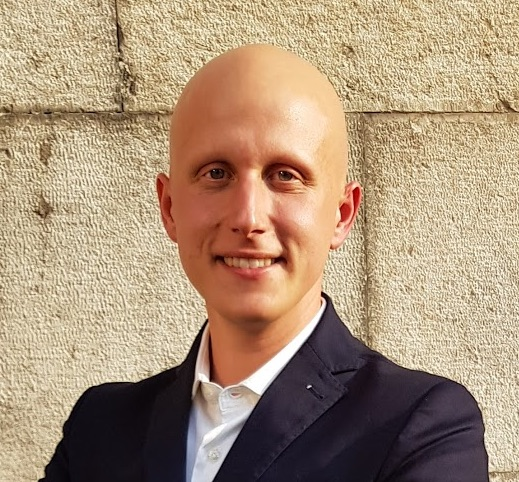
\includegraphics[width=0.8\columnwidth]{matteofico.jpg}\\[\baselineskip] % Your photo
\small % Smaller font size
Matteo Fico \\ % Your name
\url{ficomatteo@gmail.com} \\ % Your email address
\url{linkedin.com/in/matteofico} \\ % Your URL
+39 338 5801268 \\ % Your phone number
\Sep % Some whitespace
\textbf{Address} \\
Via E.Fermi 51 \\ % Address 1
41124, Modena \\ % Address 2
Italy \\ % Address 3
\vfill % Whitespace under this block to push it up under the photo
\end{flushright}
}

%----------------------------------------------------------------------------------------

\begin{document}

\userinformation % Print your information in the left column

\framebreak % End of the first column

%----------------------------------------------------------------------------------------
%	HEADING
%----------------------------------------------------------------------------------------

\cvheading{Matteo Fico} % Large heading - your name

\cvsubheading{Software Engineer} % Subheading - your occupation/specialization

%----------------------------------------------------------------------------------------
%	ABOUT ME
%----------------------------------------------------------------------------------------

\aboutme{About Me}{
	I describe myself as a thoughtful and balanced person, my focus has always been doing my job the best way possible in order to reach results. 
	
		I think good communication, reliability and punctuality are the most important values in teamwork.
	
	I try to improve my professional and personal skills everyday.
	
	I'm curious about new technologies and I've always been passionate about computer science.
						
	   }
\Sep

%----------------------------------------------------------------------------------------
%	EDUCATION
%----------------------------------------------------------------------------------------

\CVSection{Education}

%------------------------------------------------

\CVItem{July 2013, Unimore, \textit{Università di Modena e Reggio Emilia}}{Bachelor Degree in  Computer Engineering}

%------------------------------------------------

\CVItem{June 2005, ITC Barozzi, \textit{Technical high school}}{Diploma in accounting,business and programming}

%------------------------------------------------

\Sep % Extra whitespace after the end of a major section

%----------------------------------------------------------------------------------------
%	EXPERIENCE
%----------------------------------------------------------------------------------------

\CVSection{Experience}

%------------------------------------------------

\CVItem{Nov 2016 - present, \textit{R\&D Computer Vision Tech}, Unitec}{
\begin{itemize}
	\item Work on the field:
	\begin{itemize}
		\item Data collection on customers machines
		\item Train customer's technicians
		\item Install and set up computer vision software and hardware
		\item Demos (ITA - ENG - ESP)
		\item Machine supervision
	\end{itemize}
	\item Office work:
	\begin{itemize}
		\item C\# Software development 
		\item Testing new features on prototype machines
		\item Remote support
		\item Data Analysis and feasibility study
		\begin{itemize}
			\item Python/Excel data analysis and fast prototyping
		\end{itemize}
	\end{itemize}
\end{itemize}
}

%------------------------------------------------

\CVItem{Aug 2013 - Nov 2016, \textit{Software Developer}, Datagraph S.r.l.}{Main developer on public accounting softwares:
\begin{itemize}
	\item OOP, SQL Development and software management
	\item MS SQL Server maintenance
	\item Remote support and helpdesk
\end{itemize}}

\CVItem{Sep 2012 - Aug 2013, \textit{Software technician}, Spin S.r.l.}{ 
\begin{itemize}
	\item Graduation thesis|"Interfacciamento di un sistema di pesatura ed etichettatura"
	\item HMI for Supervisory Control and Data Acquisition.
\end{itemize}}


%----------------------------------------------------------------------------------------
%	NEW PAGE DELIMITER
%	Place this block wherever you would like the content of your CV to go onto the next page
%----------------------------------------------------------------------------------------

\clearpage % Start a new page

\userinformation % Print your information in the left column

\framebreak % End of the first column

\Sep % Extra whitespace after the end of a major section

%----------------------------------------------------------------------------------------
%	IT SKILLS
%----------------------------------------------------------------------------------------

\CVSection{IT Skills}

%------------------------------------------------

\CVItem{Programming}
{C\#, Python}

%------------------------------------------------

\CVItem{DBMS}
{MS SQL, MySQL}

%------------------------------------------------

\CVItem{Web}
{HTML, CSS}

%------------------------------------------------

\CVItem{Source Control}
{Mercurial, GIT, SVN}

%------------------------------------------------

\CVItem{OS}
{Windows, Mac Os X, Unix/Linux}

%----------------------------------------------------------------------------------------
%	PERSONAL SKILLS
%----------------------------------------------------------------------------------------

\Sep % Extra whitespace after the end of a major section

\CVSection{Personal Skills}

\CVItem{Problem-solving and decision-making}{Both improved working on the field}

\CVItem{Team-work}{Enhanced working on complex projects}

\CVItem{Adaptability}{Observation and eager to learn are helping me adapting}

\CVItem{Punctuality}{Be on time is a form of respect for other people}

\CVItem{Creativity}{I like graphic design and I'm passionate about UI/UX design }

%------------------------------------------------

\Sep % Extra whitespace after the end of a major section

\CVSection{Languages}

%------------------------------------------------

\CVItem{Italian}{Native} 

\CVItem{English}{Professional working}

\CVItem{Spanish}{Professional working}

\CVItem{French}{Elementary}

\Sep

%----------------------------------------------------------------------------------------
%	INTERESTS
%----------------------------------------------------------------------------------------

\CVSection{Interests}

%------------------------------------------------

\CVItem{Professional}{Data Analysis, Software Management, UX/UI, Machine Learning}

\CVItem{Personal}{Photography, travel, music, cooking, hiking}

%------------------------------------------------

\Sep % Extra whitespace after the end of a major section

%----------------------------------------------------------------------------------------


\end{document}


